\documentclass{article}
\title{Computer simulations of Stochastic Processes}
\author{Adam Janik}

\usepackage{amsmath}

\usepackage{ifthen,xcolor}
\newlength{\tabcont}

\newcommand{\tab}[1]{%
\settowidth{\tabcont}{#1}%
\ifthenelse{\lengthtest{\tabcont < .25\linewidth}}%
{\makebox[.25\linewidth][l]{#1}\ignorespaces}%
{\makebox[.5\linewidth][l]{\color{red} #1}\ignorespaces}%
}%

\usepackage{listings}
\usepackage{color}
\usepackage{graphicx}

\definecolor{dkgreen}{rgb}{0,0.6,0}
\definecolor{gray}{rgb}{0.5,0.5,0.5}
\definecolor{mauve}{rgb}{0.58,0,0.82}

\lstset{frame=tb,
  language=Matlab,
  aboveskip=3mm,
  belowskip=3mm,
  showstringspaces=false,
  columns=flexible,
  basicstyle={\small\ttfamily},
  numbers=none,
  numberstyle=\tiny\color{gray},
  keywordstyle=\color{blue},
  commentstyle=\color{dkgreen},
  stringstyle=\color{mauve},
  breaklines=true,
  breakatwhitespace=true,
  tabsize=4
}

\newcommand\xput[2][0.5]{%
    \rule{#1\linewidth}{0pt}\makebox[0pt][c]{#2}\hfill}


\begin{document}
	\pagenumbering{gobble}
	\maketitle
	\newpage
	\pagenumbering{arabic}
	
	\section{Introduction}
	In this report we are going to discuss and present some aspects regarding simulating stochastic processes. A couple of scripts has been attached to this document - they were used to produce plots and results in this report.
	\section{Stable distribution}
	In particular, we will discuss here stable distributions - a class of probability distributions, that allow skewness and heavy tails, and so have a lot of interesting mathematical properties, as well as many applications in finance, insurance mathematics, biology and many more.
	In general, an univariate stable random variables are characterized by four parameters:
	\begin{itemize}
	\item $\alpha$ - the most important one, called index of stability
	\item $\sigma$ - scale parameter
	\item $\beta$ - skewness parameter
	\item $\mu$ - shift parameter
	\end{itemize}
	Those parameters will be discussed later, here we can mention that if we want to receive Gaussian distribution, we put $\alpha = 2$, $\beta = 0$, and so $\mu$ will be mean and $\sigma$ - standard deviation.
	\subsection{Definition}
	We define $X$ as stable distribution if it holds the following property\footnote{Nolan J. P., "Stable Distributions. Models for Heavy Tailed Data", http://academic2.american.edu/~jpnolan/stable/stable.html}
	\begin{equation}
	aX_1+bX_2 \stackrel{d}{=} cX + d
	\end{equation}
	where $a, b$ and $c$ are positive, $d\in R$ and $X_1, X_2$ are independent copies of $X$.
	However, there is also another representation of stable random variable; we can say, that random variable $X$ is stable if and only if $X \stackrel{d}{=} aZ + b$ witch $Z$ being random variable with characteristic function:
	\begin{equation}
		\mathbf{E} \exp(i\mu Z) = \begin{cases}
		\exp(|\mu|^\alpha[1-i\beta \tan\frac{\pi \alpha}{2}(\mbox{sign}\mu)]) & \alpha \neq 1 \\
		\exp(|\mu|[1+i\beta \frac{2}{\pi} (\mbox{sign}\mu) \log |\mu|]) & \alpha = 1
		\end{cases}
	\end{equation}
In this equation we have $0<\alpha \leq 2$ and $-1 \leq \beta \leq 1$, $a$ must be different than $0$ and $b$ is a real number.\\
A more precise description and derivation of stable distribution can be found in dedicated literature\footnote{Samorodnitsky G, Taqqu M.S, "Stable Non-Gaussian Random Processes"}. Here we are going to discuss some aspect of simulations and properties.

	\subsection{Simulation and properties}
	A simple function (for Matlab language) to simulate stable random variables\footnote{Borak, Hardle, Weron, 2005} has been attached to this report. Crucial for us is to check if it works correctly and investigate properties of the simulated distribution. Fortunately, a there is a very well-known program\footnote{http://academic2.american.edu/~jpnolan/stable/stablec.exe}, written by John P. Nolan, available on his website. With it's help, we will be able to test our function.
	\subsubsection{Testing for correctness of the function}
	Let's make four calls of the function to generate data, and then check if with Nolan's program:
	\begin{lstlisting}
	gaussian = stable(2, 0, 1, 0, 100000);$
	cauchy = stable(1, 0, 1, 0, 100000);$
	levy = stable(0.5, 1.0, 1, 0, 100000);$
	distr = stable(1.3, 0.3, 2, -5, 100000);$
	\end{lstlisting}
	As a result, we obtained four samples of stable distribution; now we can check them with Nolan's program. We choose each time maximum likelihood estimators of parameters method to get parameters based on sample. \\
	
	For a variable \textit{gaussian} the output is:
	\begin{lstlisting}
	 Stable model with maximum likelihood estimator
	 
  Initial quantile estimate of S0 parameters
         alpha     beta      gamma         delta
      2.000000}  0.000000    1.00421       0.911811E-03   
\end{lstlisting}       
   
For a variable \textit{cauchy} the output is:
\begin{lstlisting}
	 Stable model with maximum likelihood estimator
	 
  Initial quantile estimate of S0 parameters
         alpha      beta      gamma         delta
      0.995880  -0.017271    1.00109       0.190453E-02
\end{lstlisting} 

For a variable \textit{levy} the output is:\\
\begin{lstlisting}
	 Stable model with maximum likelihood estimator
	 
  Initial quantile estimate of S0 parameters
         alpha      beta      gamma         delta
      0.506668  0.815349    1.31190       1.17643   
\end{lstlisting} 

For a variable \textit{distr} the output is:
\begin{lstlisting}
	 Stable model with maximum likelihood estimator
	 
  Initial quantile estimate of S0 parameters
         alpha      beta      gamma         delta
      1.306687  0.311575    1.99745       -6.18514   
\end{lstlisting}  
We can say here now, that estimation goes worse as $\alpha$ is going lower - especially for $\mu$ (or - in other sources $\sigma$) parameter; we should be careful when we are saying something about shift parameter, when we operating on the low-$\alpha$ samples.

	\begin{figure}[h]
		\xput[0.5]{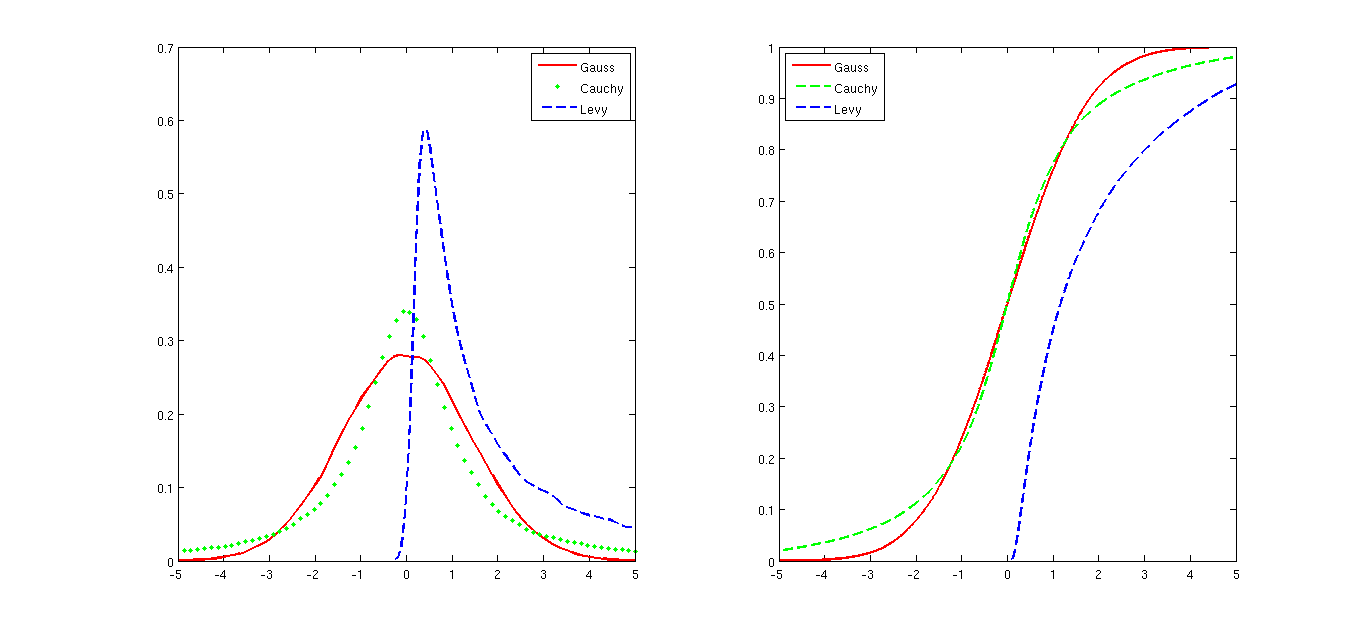
\includegraphics[width=1.7\linewidth]{gauss_cauchy_levy}}
		
		\caption{Simulated three important distributions with $\alpha = 2, 1, 0.5$}
	\end{figure}

\subsection{Description of the parameters}
In this subsection we will discuss each of the parameters and how changing them, impacts obtained sample.
\subsubsection{$\alpha$ parameter}
Mentioned before, index of stability is often referred as the most important one. On the Figure 2 three samples have been presented, to illustrate how stable distribution behave with decreasing $\alpha$. We can see that three things occur to the density: peak gets higher, the region flanking peak get lower, and - what makes stable distribution such important and interesting - the tails gets heavier.\\
As shown in the next section, $\alpha$ affects heavily other parameters.

	\begin{figure}[h]
		\xput[0.5]{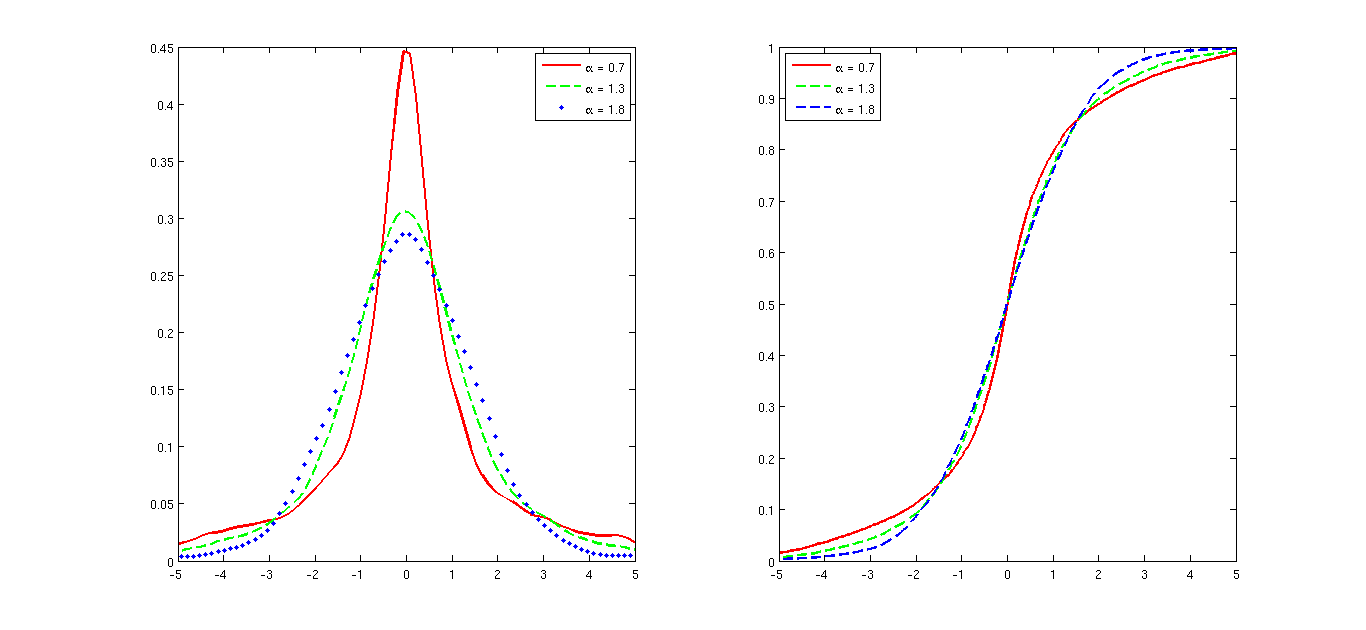
\includegraphics[width=1.7\linewidth]{stable_param_alpha}}
		
		\caption{Stable distribution pdf and empirical cdf for $\alpha = 0.7, 1.3, 1.8$}
	\end{figure}

\subsubsection{$\beta$ parameter}
Three different plots for different simulated samples will be needed, to show how $\beta$ influence our distribution.

Figure 3 allows us to see, that with increasing $\beta$, the distribution becomes more and more skewed to the right (in case of $\beta$ negative, we would see similar behavior, but to the left side)
	\begin{figure}[h]
		\xput[0.5]{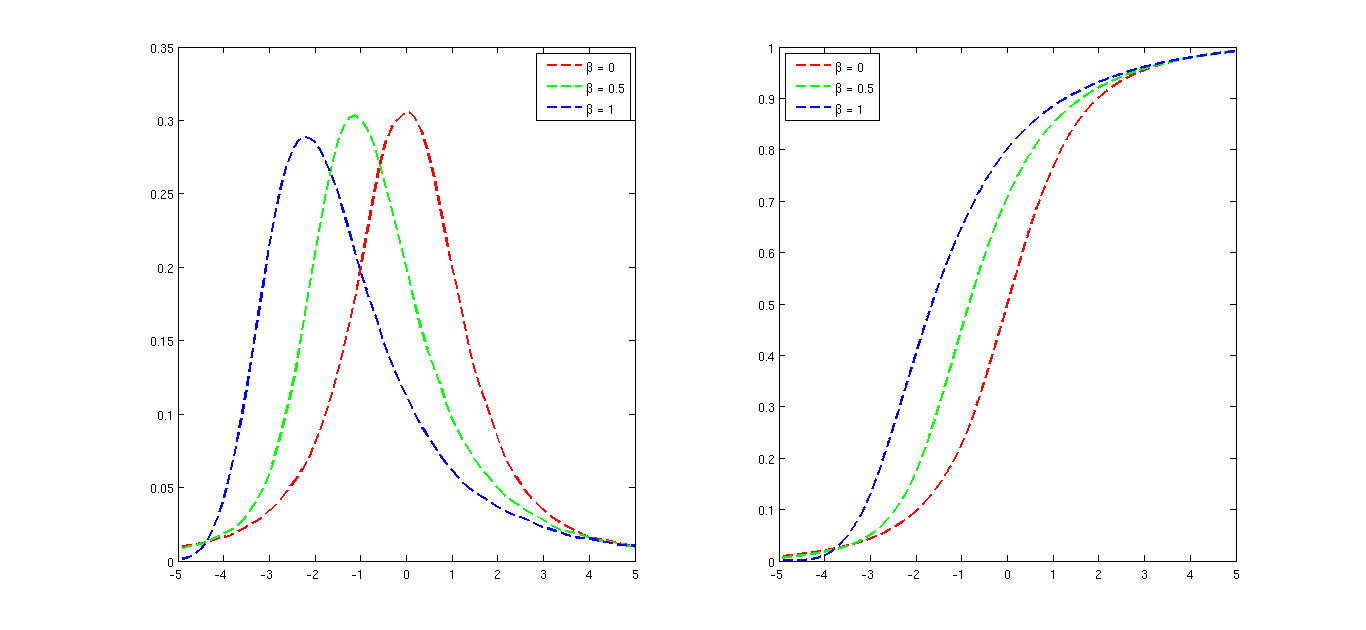
\includegraphics[width=1.5\linewidth]{stable_param_beta13}}
		
		\caption{Stable distribution pdf and empirical cdf for $\alpha = 1.3$ and $ beta = 0, 0.5, 1$}
	\end{figure}
\newpage
In Figures 4 and 5 $\beta$ varying in the same way, but samples has been simulated for $\alpha = 1$ and $\alpha = 0.7$ respectively.
	\begin{figure}[h]
		\xput[0.5]{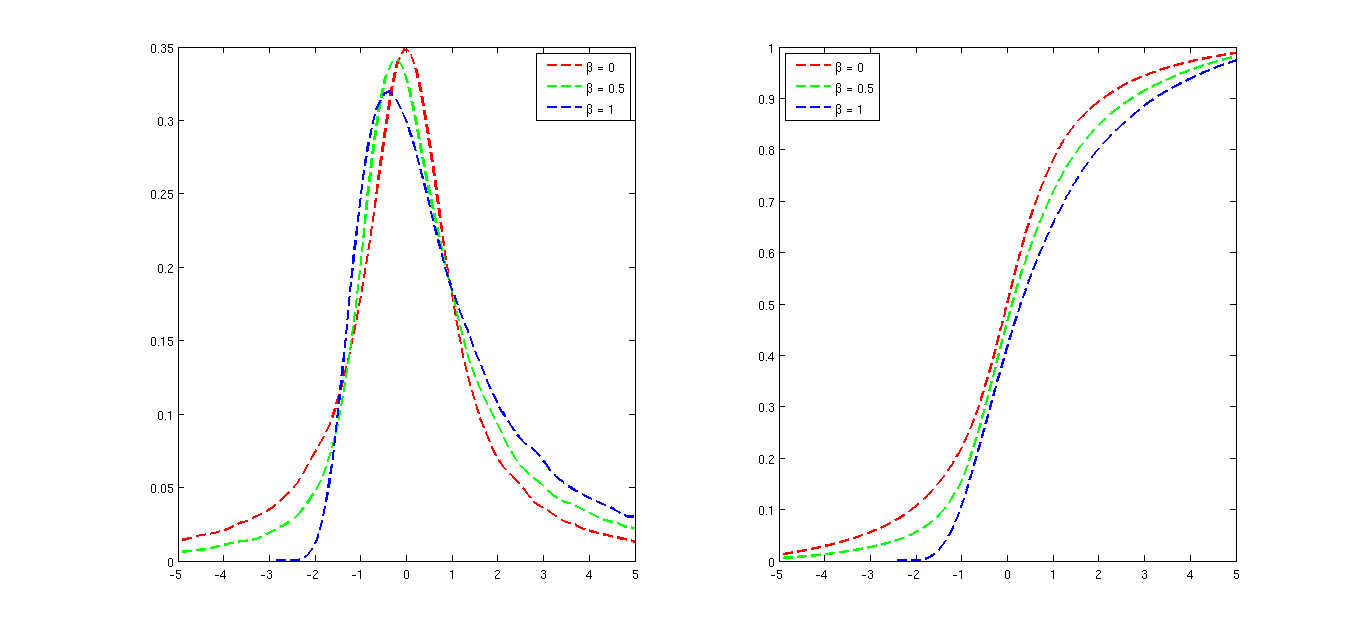
\includegraphics[width=1.5\linewidth]{stable_param_beta10}}
		
		\caption{Stable distribution pdf and empirical cdf for $\alpha = 1$ and $ beta = 0, 0.5, 1$}
	\end{figure}
	
	\begin{figure}[h]
		\xput[0.5]{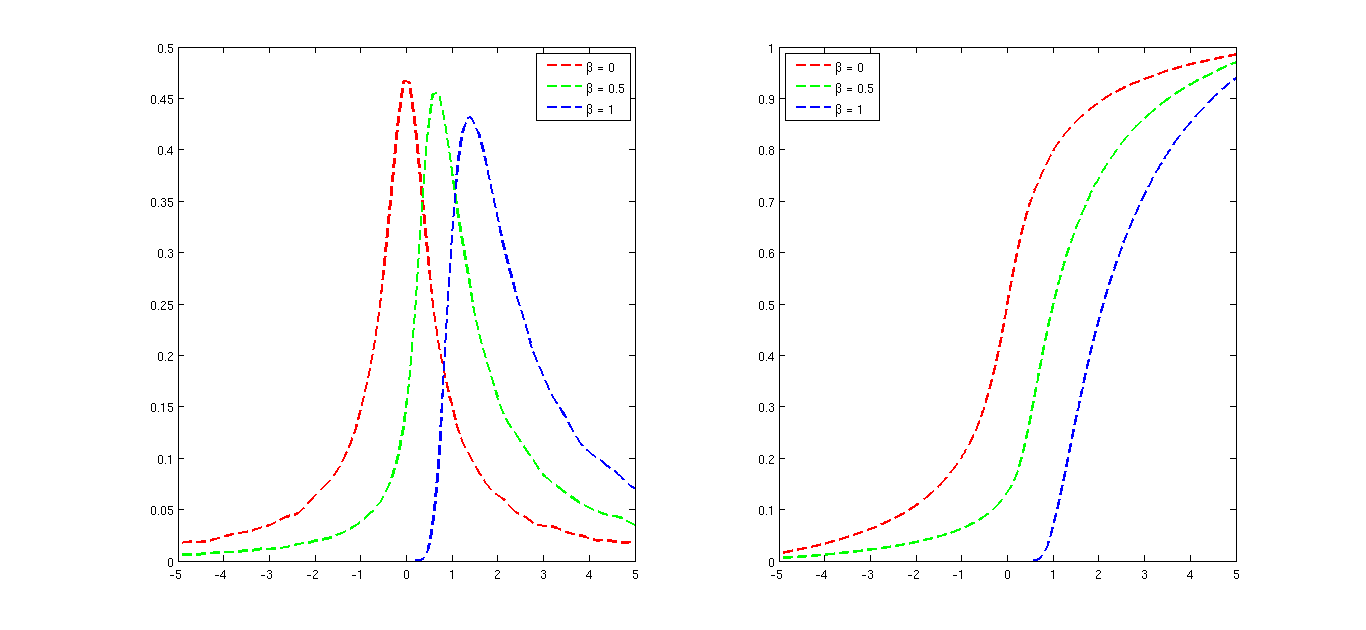
\includegraphics[width=1.5\linewidth]{stable_param_beta07}}
		
		\caption{Stable distribution pdf and empirical cdf for $\alpha = 0.7$ and $ beta = 0, 0.5, 1$}
	\end{figure}
We see that with decreasing $\alpha$, $\beta$ becomes more and more significant, making distribution more and more skewed, until it reach 1 (-1) - then we say that distribution is \textit{totally skewed to the right (left)}. It can also be shown, that for $\alpha < 1$ and $|\beta| = 1$ the whole weight is in one of the tails (depending if $\beta$ is negative or positive).
\clearpage
\subsection{Properties}
Here we discuss some of the commonly known properties\footnote{Samorodnitsky G, Taqqu M.S, "Stable Non-Gaussian Random Processes"} of the stable distributions.
\subsubsection{Property 1}
First, we are going to study the following property\footnote{Samorodnitsky G, Taqqu M.S, "Stable Non-Gaussian Random Processes"}:
\subparagraph{Property 1}
\textit{Let $X_1$ and $X_2$ be independent stable random variables, $X_i \sim S_\alpha(\beta_i, \sigma_i, \mu_i)$, $i = 1,2$. Then $X_1 + X_2 \sim S_\alpha(\beta, \sigma, \mu)$, with: }
\begin{equation}
\sigma = (\sigma_1^\alpha + \sigma_2^\alpha)^{1/\alpha}, \qquad \mu = \mu_1 + \mu_2, \qquad \beta = \frac{\beta_1\sigma_1^\alpha + \beta_2\sigma_2^\alpha}{\sigma_1^\alpha + \sigma_2^\alpha}
\end{equation}
Following code has been ran to simulate two samples:

\begin{lstlisting}
alpha = 1.8;
mu1 = 1; mu2 = 0.5;
sigma1 = 0.5; sigma2 = 0.3;
beta1 = 0.3; beta2 = 0.8;
sigma = ( sigma1^alpha + sigma2^alpha )^(1/alpha);
beta = ( beta1*(sigma1^alpha) + beta2*(sigma2^alpha) ) / ( sigma1^alpha + sigma2^alpha );
mu = mu1 + mu2;

X1 = stable(alpha, beta1, sigma1, mu1, 10000000);
X2 = stable(alpha, beta2, sigma2, mu2, 10000000);
X = X1 + X2;
save X.txt X -ascii;
\end{lstlisting}
Values computed according to formula above are as follows: $sigma = 0.6025, \beta = 0.4425, \mu = 1.5000$; output from Nolan's program, checking parameters:
\begin{lstlisting}
  Initial quantile estimate of S0 parameters
         alpha      beta      gamma         delta
      1.800206  0.452978   0.602503        1.41195 
\end{lstlisting}   
The largest difference between theoretical and simulated value is at $\delta$ (or $\mu$) parameter; however, taking consideration, that in the previous examples it was most variable parameter, we can say that property holds.

\subsubsection{Property 2}
Another property, that we can easily check is the following one
\subparagraph{Property 2}
For any $0 < \alpha < 2$,
\begin{equation}
X \sim S_\alpha(\beta, \sigma, \mu) \iff -X \sim S_\alpha(-\beta, \sigma, \mu)
\end{equation}

\begin{lstlisting}
alpha = 1.8; mu = 0; sigma = 1; beta = 0.7;
X = stable(alpha, beta, sigma, mu, 1000000);
X = -X; save X.txt X -ascii;
\end{lstlisting} 
And again we check with the Nolan's program:
\begin{lstlisting}
  Initial quantile estimate of S0 parameters
         alpha      beta      gamma         delta
      1.802983 -0.716207    1.00018       0.230816 
\end{lstlisting}
We can say that property holds
\end{document}
	